\documentclass[compress, aspectratio=169]{beamer}

%presentation layout

\mode<presentation>
{
	\usetheme{Berlin}
	% \usecolortheme{dove}
	\setbeamercolor{structure}{bg=white,fg=black}
	\setbeamercolor{normal text}{bg=white,fg=black}
	\setbeamercolor{titlepage}{bg=white,fg=black}
	\setbeamercolor{titlelike}{bg=white,fg=black}
	\setbeamercolor{palette primary}{bg=white}
	\setbeamercolor{palette secondary}{bg=gray, fg=white}
	\setbeamercolor{palette tertiary}{bg=gray, fg=white}
	\setbeamercolor{palette quarternary}{bg=white}
	\setbeamercovered{transparent}
	\useinnertheme{rectangles}
	%\usefonttheme{serif}
}

\setbeamertemplate{navigation symbols}{}

%loading packages
\usepackage[ngerman]{babel}
\usepackage[T1]{fontenc}
\usepackage[utf8]{inputenc}
\usepackage{graphicx}
\graphicspath{{img/}}
\usepackage{amsmath}
\usepackage{framed}
\usepackage{caption}
\usepackage{subcaption}
\usepackage{multicol} 
\usepackage{xcolor}

\usepackage{qrcode}

\definecolor{light-gray}{gray}{0.97}

% vorgeplaenkel
\title[Anfangsplenum]{Anfangsplenum}

\author{Ständiger Ausschuss aller Physikfachschaften}

\institute[Zusammenkunft aller Physikfachschaften]

\date{12. Mai 2021}

\subject{Anfangsplenum der OstseeZaPF 2021}

\begin{document}
	
	\section{Begrüßung}
	
	{
		\setbeamercolor{background canvas}{bg=light-gray}
		\begin{frame}
			\begin{figure}
				\centering
				
\includegraphics[height=5.5cm]{LOGO.png}
			\end{figure}
			\centering
			\textbf{Willkommen zur OstseeZaPF 2021!}
		\end{frame}
	}
	
	\begin{frame}{How to Plenum}
		Diese ZaPF ist eine ZaPF! Und das ist nicht mal tautologisch.\\
		$\Rightarrow$ Die Geschäftsordnung für Plenen der ZaPF findet wieder Anwendung.
		
		\vspace{.5cm}
		Meldungen über den Chat:
		\begin{itemize}
			\item$\quad$\textbf{!}$\quad$ \ \ Meldung
			\item$\quad$\textbf{!!}$\quad$ \ Verständnisfrage
			\item$\quad$\textbf{!!!}$\quad$ Geschäftsordnungs-Antrag
		\end{itemize}
		\vspace{.5cm}
		Nennt zu Beginn eines Redebeitrags bitte Name und Uni.
	\end{frame}
	
	\section{Formalia}
	
	\begin{frame}{Bestimmung der Redeleitung}
		\centering
		Vorgeschlagene Redeleitung:
		\vspace{.5cm}
		
		\hspace{0.1\textwidth}
		\begin{minipage}{.3\textwidth}
			\begin{figure}
				\begin{minipage}[c]{.655\textwidth}
					
\includegraphics[height=0.5\textheight]{sean.jpg}
				\end{minipage} \hfill
				\begin{minipage}[c]{.632\textwidth}
					\caption*{Sean Bonkowski \\ Uni Bonn}
				\end{minipage}
			\end{figure}
		\end{minipage}
		\hspace{0.1\textwidth}
		\begin{minipage}{0.4\textwidth}
			\begin{figure}
				\begin{minipage}[c]{.65\textwidth}
					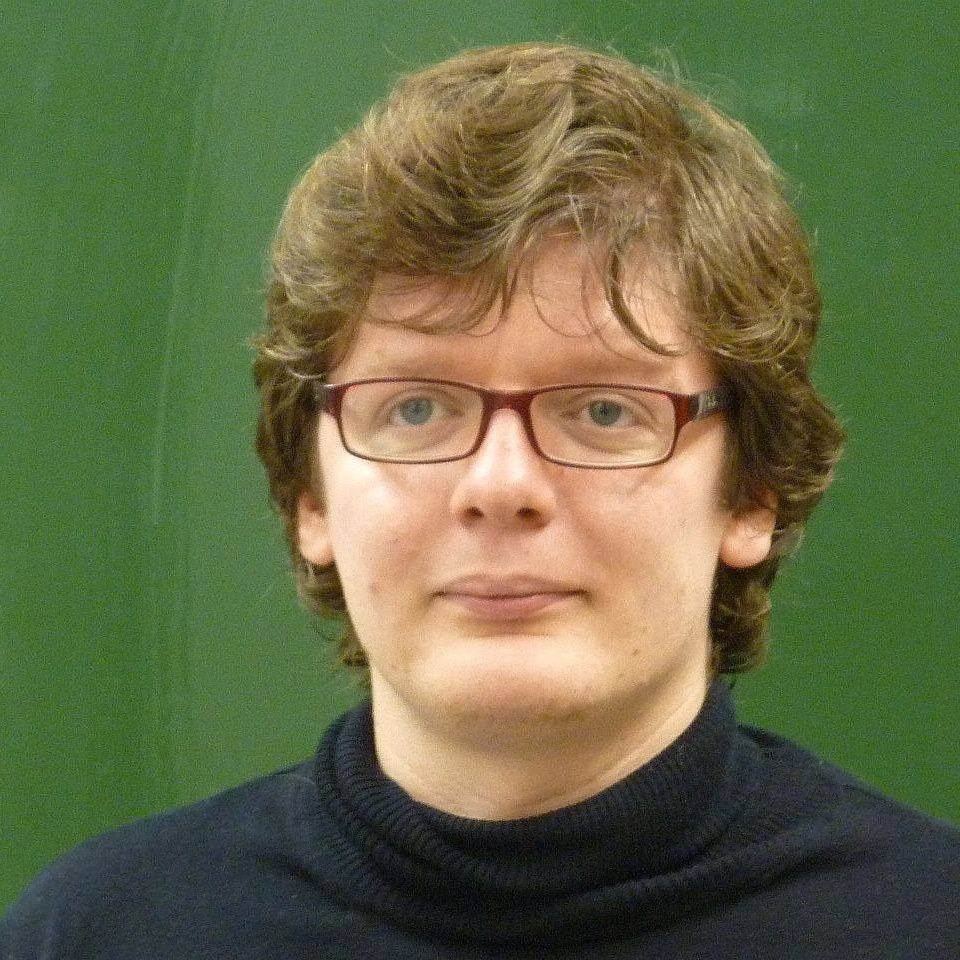
\includegraphics[height=0.5\textheight]{philipp.jpg}
				\end{minipage} \hfill
				\begin{minipage}[c]{.632\textwidth}
					\caption*{Philipp Jaeger\\ Alumni}
				\end{minipage}
			\end{figure}
		\end{minipage}
		\hspace{0.1\textwidth}
	\end{frame}
	
	\begin{frame}{Bestimmung der Protokollführung}
		Vorgeschlagene Protokollführung:
		%Hier noch die Protokollanten einfügen
		\begin{itemize}
			\item Anna Summers 
			\item Gabriel Sellge
			\item Leon Nutzinger
		\end{itemize}
	\end{frame}
	
	\begin{frame}{Feststellung der Beschlussfähigkeit} %Warten auf Feedback vom TOPF zum Stand des Tools und dann fertig schreiben
		Geschäftsordnung (§4): \textit{Die Beschlussfähigkeit für Abstimmungen und Personenwahlen ist gegeben, wenn zwanzig Physikfachschaften im Plenum anwesend sind.}\vspace{.5cm}
		
		Verfahrensvorschlag: Nutzung eines Abstimmungstools, bei dem der Zugang über das Fachschaftstoken geregelt wird.\vspace{.5cm}
		
		Feststellung der Beschlussfähigkeit: Bitte meldet euch jetzt im Abstimmungstool an und bestätigt eure Anwesenheit.
	\end{frame}
	
	%\begin{frame}{Es wird auch wieder analog!}
	%    \begin{figure}
	%        \centering
	%        \includegraphics[height=3.5cm]{Zapf_logo_zapfig2020.png}
	%        \includegraphics[height=4cm]{LOGO-OSTSEEZAPF20180317_korrigiert.png}
	%        \includegraphics[height=3.2cm]{logo_goettingen.png}
	%    \end{figure}
	%    \vspace{0.25cm}
	%    \centering
	%    \large Viel Erfolg und vielen Dank an alle ausrichtenden Fachschaften!
	%\end{frame}
	
	%\section{Allgemeine Infos}
	%
	%\begin{frame}{Zum Eröffnungstreffen}
	%    \begin{itemize}
	%        \item Meldungen über den \glqq Melden\grqq-Status oder über den Chat
	%        \item Für Redebeiträge könnt ihr die Bildübertragung einschalten
	%        \item Kein offizielles Plenum, also nicht gebunden an die GO
	%        \item Handelt bitte trotzdem in ihrem Sinne, verhaltet euch nett und rücksichtsvoll!
	%        \item Live-Protokoll unter protokolle.zapf.in/s/protokoll$\_$eroeffnungstreffen
	%    \end{itemize}
	%
	%
	%\end{frame}
	%
	%\begin{frame}{Das Team fürs Eröffnungstreffen}
	%        \begin{itemize}
	%        \item Moderation: Peter, Andy
	%        \item Redeliste $\&$ Chat: ChrisPi, Daniela
	%        \item Protokoll: Anna, Tobi, Vicky, Hannah
	%        \item AK-Planung: Vicky
	%        \item IT-Support: Timo, Sean
	%    \end{itemize}
	%\end{frame}
	
	
	
	\begin{frame}{Beschluss der Tagesordnung}
		\begin{multicols}{2}
			\begin{enumerate}
				\item Begrüßung
				\item Formalia
				\begin{enumerate}
					\item Bestimmung der Redeleitung
					\item Bestimmung der Protokollführung
					\item Feststellung der Beschlussfähigkeit
					\item Beschluss der Tagesordnung
				\end{enumerate}
				\item Infos der Orga
				\item Wahl der Vertrauenspersonen
				\item Vorstellung der Arbeitskreise
				\item Gremienberichte
				\begin{enumerate}
					\item StAPF
					\item TOPF
					\item KomGrem
					\item ZaPF e.V. Vorstand
				\end{enumerate}
				\item Kommende ZaPFen
				\item Festlegung der Arbeitskreise
				\item Sonstiges
			\end{enumerate}
		\end{multicols}
	\end{frame}
	
	\section{Infos der Orga}
	

	
	\section{Infos der Orga}
	
\begin{frame}{Wichtige Links und Mail-Adressen}
\begin{itemize}
        \item \url{https://play.workadventu.re/@/zapf/zapf\_world/hro\_amphitheater}  \\
        \begin{center}
            \qrcode{https://play.workadventu.re/@/zapf/zapf\_world/hro\_amphitheater}
        \end{center}
        \item \url{https://ostsee.zapf.in/wo-ist-was/}   \\
        \begin{center}
            \qrcode{https://ostsee.zapf.in/wo-ist-was/}
        \end{center}
        \item Orga-Mail: \url{zapf.physik@uni-rostock.de}
        \item Teilnehmikaliste: \url{ostseezapf2021@uni-rostock.de}
\end{itemize}
\end{frame}

\begin{frame}{Digitale Welt}
\begin{itemize}
    \item Treffen von bis zu vier Teilnehmika unterwegs
    \item AK-Räume (gelbe Türen)
    \item Ruhe-Räume (blau)
    \item Orga-Büro (grün)
    \item Kleingruppenarbeitsräume (lila)
    \item Raum für Vertrauenspersonen (gelb)
    \item Geheime Karte: Partykeller
    \item Erkundet die Welt und seid lieb zu einander
\end{itemize}

\end{frame}
	\begin{frame}{Ablaufplan der Ostsee-ZaPF}
		\begin{figure}
			\centering
			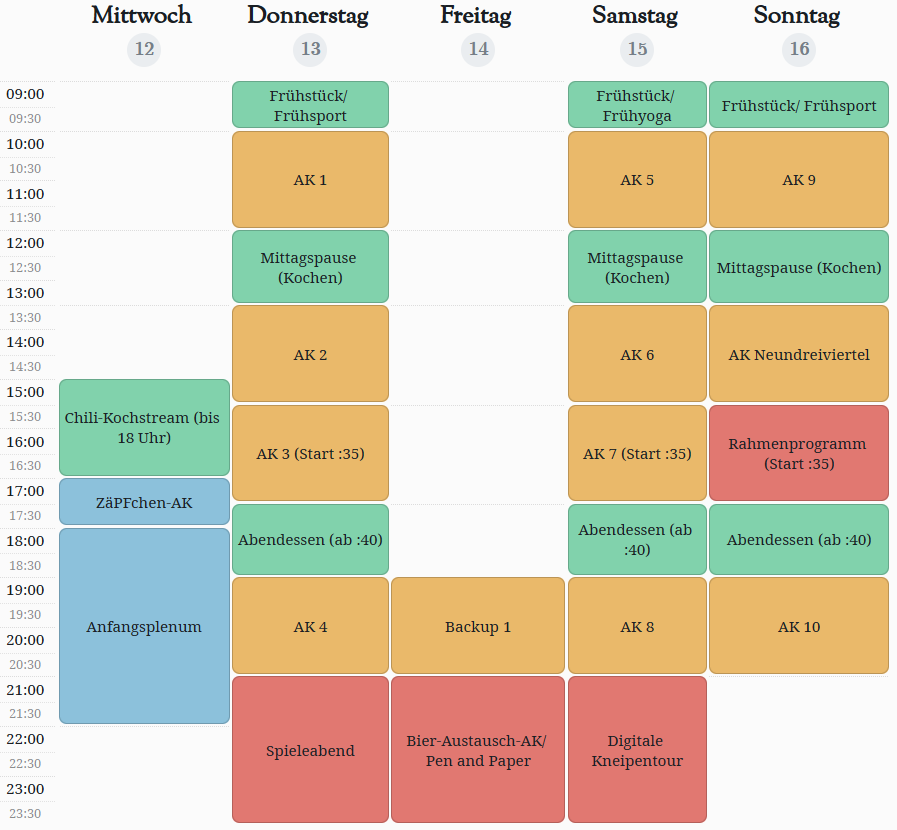
\includegraphics[height=5.8cm]{Woche1.png}
		\end{figure}
	\end{frame}
	
	\begin{frame}{Ablaufplan der Ostsee-ZaPF}
		\begin{figure}
			\centering
			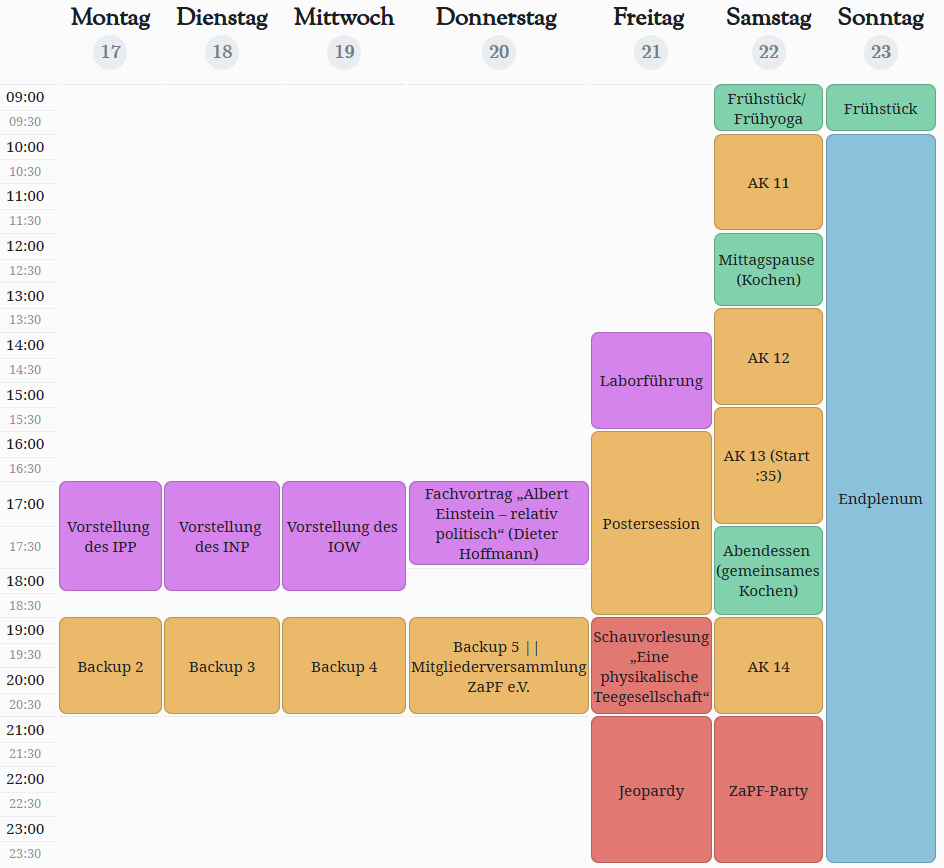
\includegraphics[height=5.8cm]{Woche2.png}
		\end{figure}
	\end{frame}


\begin{frame}{Vertrauenspersonen der Orga}
\begin{tabular}{ll}
  \textbf{Wanda:}  &  Telegram: @WWinterkind \\
    & Mail: \url{wanda.witte@uni-rostock.de} \\

   \textbf{Jona:} & Telegram: @Jona\_telegram \\
  & Mail: \url{jonathan.mette@uni-rostock.de} \\
  
\end{tabular} 
\vspace{.5cm}

\hspace{0.1\textwidth}

\begin{minipage}{.3\textwidth}
	\begin{figure}
		\begin{minipage}[c]{.655\textwidth}
			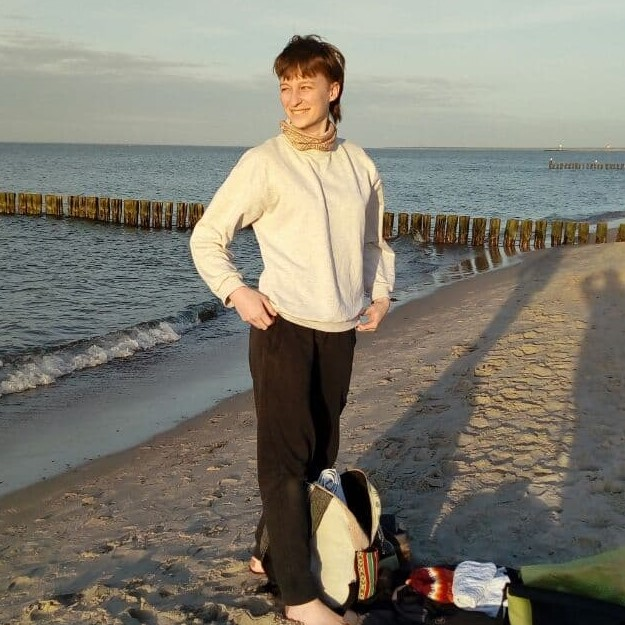
\includegraphics[height=0.5\textheight]{wandaw.jpg}
		\end{minipage} \hfill
		\begin{minipage}[c]{.632\textwidth}
			\caption*{Wanda Witte}
		\end{minipage}
	\end{figure}
\end{minipage}
\hspace{0.1\textwidth}
\begin{minipage}{0.4\textwidth}
	\begin{figure}
		\begin{minipage}[c]{.65\textwidth}
			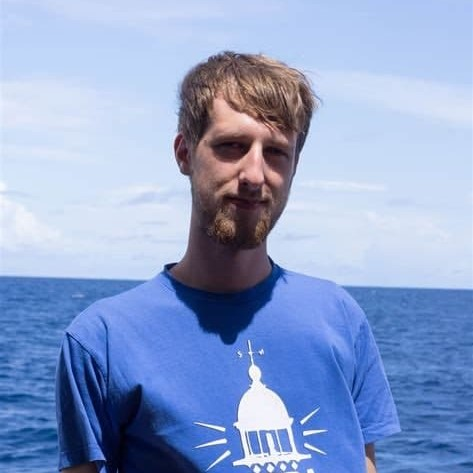
\includegraphics[height=0.5\textheight]{jonam.jpg}
		\end{minipage} \hfill
		\begin{minipage}[c]{.632\textwidth}
			\caption*{Jonathan Mette}
		\end{minipage}
	\end{figure}
\end{minipage}
\hspace{0.1\textwidth}

\begin{figure}[h!]
       \centering
       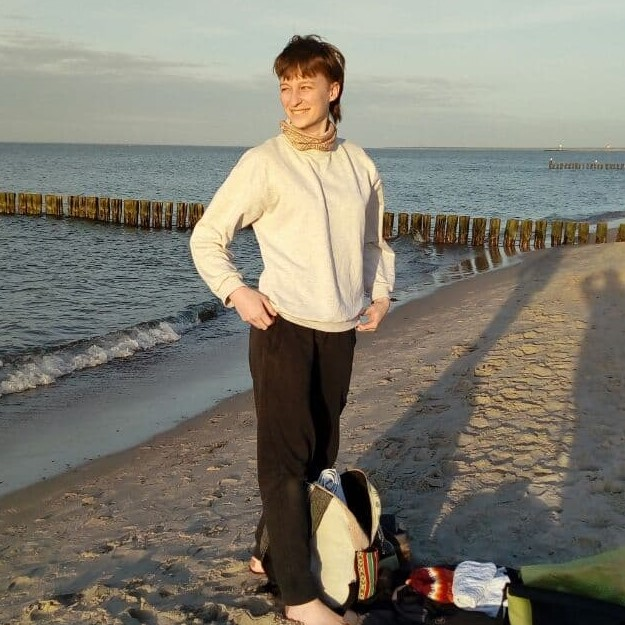
\includegraphics[width=0.4\textwidth]{wandaw.jpg}
       \hfill
       \centering
       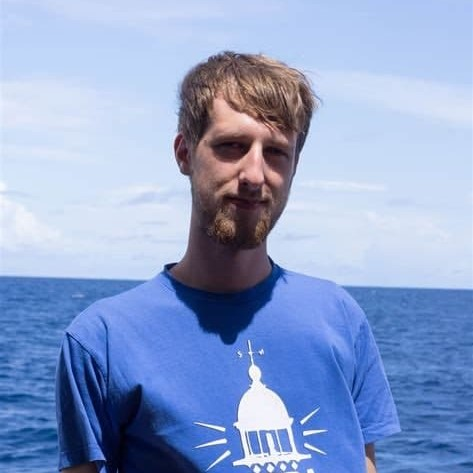
\includegraphics[width=0.4\textwidth]{jonam.jpg}
   \end{figure}   
\end{frame}

\begin{frame}{Rahmenprogramm}
\begin{tiny}
    \begin{table}[h]
        \centering
        \begin{tabular}{lll}
             \textbf{Woche I}& & \\
             Do, \(13.05.\) \(9\) Uhr & Frühsport & Digitale Welt, Raum 5 EG HRO\\
             Do, \(13.05.\) \(21\) Uhr & Spieleabend & Digitale Welt, Partykeller\\
             & & \\
             Fr, \(14.05.\) \(21\) Uhr & Bieraustausch-AK & Digitale Welt, Partykeller\\
             Fr, \(14.05.\) \(21\) Uhr & Pen \& Paper Runde & Nach Anmeldung\\             
             & & \\
             Sa, \(15.05.\) \(9\) Uhr & Frühyoga & Digitale Welt, Raum 5 EG HRO\\             
             Sa, \(15.05.\) \(21\) Uhr & Kneipentour & Digitale Welt, Foyer Rostock\\        
             & &  \\
             So, \(16.05.\) \(21\) Uhr & Frühsport-AK & Digitale Welt, Raum 5 EG HRO\\
             & & \\
             \textbf{Woche 2} & &\\
             Mo, \(17.05.\) \(17\) Uhr & Vorstellung IPP & Digitale Welt, Raum 3 EG HGW\\
             Di, \(18.05.\) \(17\) Uhr & Vorstellung INP & Digitale Welt, Raum 3 EG HGW\\
             Mi, \(19.05.\) \(17\) Uhr & Vorstellung IOW & Digitale Welt, Raum 3 EG HGW\\
             Do, \(20.05.\) \(17\) Uhr & Fachvortrag \glqq Albert Einstein - relativ politisch\grqq & t.b.a\\
             Fr, \(21.05.\) \(14\) Uhr & Laborführungen & t.b.a\\
             Fr, \(21.05.\) \(19\) Uhr & Schauvorlesung & t.b.a\\
             Fr, \(21.05.\) \(21\) Uhr & Jeopardy & Digitale Welt, Raum 1 EG HRO\\
             Sa, \(22.05.\) \(9\) Uhr & Frühyoga & Digitale Welt, Raum 5 EG HRO\\
        \end{tabular}
    \end{table}
\end{tiny}
\end{frame}

\begin{frame}{Rahmenprogramm}
    \begin{footnotesize}
    \textbf{Fotochallenge}\\
    Mache Fotos zu 7 Themen. Die schönsten Fotos jeder Kategorie werden demokratisch bestimmt.
    Veröffentlicht auf \url{https://talk.zapf.in/t/ostseezapf2021-fotochallenge/370}\\
    \textbf{Buddy-Bingo}\\ 
    Kannst du das Bingo vervollständigen indem du ZaPFika findest, die die Kriterien erfüllen? \url{https://talk.zapf.in/t/buddy-bingo/380}\\
    \textbf{Entenraten}\\
    Wie viele Enten findest du in unserer digitalen Welt?
    Schreibe es auf \url{https://talk.zapf.in/t/entenraten/373}.\\
    Gotta catch ‘em all!\\
    \textbf{Spaziergehbuddies}\\
    Trefft Leute zum Spazieren gehen (digital und in echt) in der Brandung des Ostseestrandes!\\
    \begin{center}
        \textbf{Es gibt Preise!}\\
        Nähere Informationen unter \url{https://ostsee.zapf.in/rahmenprogramm/}
    \end{center}
    \end{footnotesize}
    
\end{frame}
	
	%\begin{frame}{Das Rahmenprogramm}
	%\begin{itemize}
	%\item Filmabend (Freitag, 06.11. - im Anschluss an dieses Plenum)
	%\item Kneipentour + Karaoke (Samstag, 07.11.)
	%\item Pen\&Paper + Online-Spieleabend (Sonntag, 08.11.)
	%\item Gamerallye (Montag bis Freitag nach den AK-Slots)
	%\item Party + Karaoke (Samstag, 14.11.)
	%\end{itemize}
	%Außerdem Frühsport um 9:00 an beiden Wochenenden!
	%\end{frame}
	
	%\begin{frame}{Technik der Digital-ZaPF}
	%    \begin{itemize}
	%    \item Teilnehmika-Mailingliste
	%    \item BigBlueButton
	%    \item Discourse-Forum
	%    \item HackMD
	%    \item Mumble
	%    \item ZaPF-Wiki
	%    \end{itemize}
	%    \vspace{0.5cm}
	%    \centering
	%    Bitte nutzt wo immer möglich die Angebote auf dem ZaPF-Server!
	%\end{frame}
	
	%\begin{frame}{Vertrauenspersonen} %Die Vertauenspersonen sobald bekannt einfügen bzw. %das Bild hochladen
	%	\begin{figure}
	%		\centering
	%		%\includegraphics[height=6cm]{VP_Plakat_Ostsee.png}
	%		%TODO
	%	\end{figure}
	%\end{frame}
	
	\section{Vorstellung der Arbeitskreise}
	\begin{frame}{Vorstellung der Arbeitskreise}
	\begin{itemize}
		\item AKs werden in der Reihenfolge der Tabelle im Wiki vorgestellt
		\item Bitte fasst euch kurz!
		\item Im Anschluss an die Vorstellung wird der Terminplan fertiggestellt (parallel zu den Gremienberichten)
		\item Wenn ihr Terminkollisionen feststellt oder kurzfristig einen AK einreichen wollt, schreibt bitte eine Mail an zapf.physik@uni-rostock.de
	\end{itemize}
\end{frame}

\begin{frame}{Arbeitskreise I}
	\begin{itemize}
		\item Mitgliederversammlung ZaPF e.V.
		\item AK Wissenschaftsrecht - Opa, Gabriel (Chemnitz)
		\item AK Klafki für die Hochschule - Amr (HU Berlin), Stefan (Köln)
		\item AK Orga-Austausch - Andy (Würzburg)
		\item AK Austausch - tbd
	\end{itemize}
\end{frame}

\begin{frame}{Arbeitskreise II}
	\begin{itemize}
		\item Selbstberichtsbewertung - Tobi (Düsseldorf)
		\item Open Source ab Universitäten - Tobi (Düsseldorf)
		\item Open Source Bildungsplattformen - Tobi (Düsseldorf)
		\item Datenschutz Videokonfernzsysteme - Tobi (Düsseldorf)
		\item Wiki Pflege - Tobi (Düsseldorf)
	\end{itemize}
\end{frame}

\begin{frame}{Arbeitskreise III}
	\begin{itemize}
		\item AK Einführung zu Mobilität und Durchlässigkeit - Fabs
		\item AK Gemeinsames PosPa zu Mobilität und Durchlässigkeit -  Fabs
		\item AK Fachschafts-Veranstaltungen - Andy (Würzburg)
		\item AK BaMa-Umfrage - Felicia (Göttingen)
		\item MeTaFa - Vicky (Alumni)
	\end{itemize}
\end{frame}

\begin{frame}{Arbeitskreise IV}
	\begin{itemize}
		\item AK Studiengang-Diagramm Erstellung - Stefan (Köln), Daniela (ehemals Frankfurt)
		\item AK NFDI - Philipp (Alumni)
		\item AK Wissenschaftliche Kariere - Philipp (Alumni)
		\item AK Wissenschaft und Gesellschaft - Philipp (Alumni)
		\item AK Mental Health Umfrage - Philipp (Alumni)
	\end{itemize}
\end{frame}

\begin{frame}{Arbeitskreise V}
	\begin{itemize}
		\item AK Nachhaltigkeit - Daniel (TUM), Katrin (TUM)	
		\item AK Lehramtsumfrage KFP - Sebbo (Heidelberg)
		\item AK Fachschaften und jDPG - Janice (Münster)
		\item Der StAPF stellt sich vor - StAPF
		\item AK Fachschaftsnachwuchs - Laura (Würzburg), Tim (Würzburg) 
	\end{itemize}
\end{frame}

\begin{frame}{Arbeitskreise VI}
	\begin{itemize}
		\item Angemessene Prüfungsformate \& Programmieren - Manu (Wien) 
		\item Hybrid Lehre - Manu (Wien), Amr (HU Berlin)
		\item AK Bayerische Hochschulgesetznovelle - Andy (Würzburg) 
		\item AK Fachschafts-Freundschaften - Andy (Würzburg), Tobi (Düsseldorf)
		\item AK Handreichung zu Mental Health - tbd 
	\end{itemize}
\end{frame}

\begin{frame}{Arbeitskreise VII}
	\begin{itemize}
		\item AK Studienführer 2.0 - Vicky (Alumni) 
		\item AK KommGrem - KommGrem 
		\item AK Lost Generation - tbd
		\item AK Ad Personam Professur und Anforderungen an Professuren - Paul (Köln)
		\item AK Austausch Lehramt - Leon (FU Berlin)
	\end{itemize}
\end{frame}

\begin{frame}{Arbeitskreise VIII}
	\begin{itemize}
		\item AK Evaluation der Lehre - Jules (Hamburg), Markus (Hamburg)
		\item Forschungsorientierte Lehre - Amr (HU Berlin)
		\item Atomwaffen, das Recht des Stärkeren und was wir dagegen in der Hand haben - Christos (ehemals Köln)
	\end{itemize}
\end{frame}

\begin{frame}{Workshops und Mindestgrößen-AKe}
	\begin{itemize}
		\item WS Einführung in die Akkreditierung - tbd
		\item Awareness-Spiel - Hannah (Alumni), Amr (HU Berlin)
	\end{itemize}
	\vspace{.5 cm}
	\begin{itemize}
		\item Freie Diskussion über berufliche (Nicht-)Perspektiven in der Forschung - Katrin (TUM)
		\item AK Austausch mit Promovierendennetzwerken - Vicky (Alumni), Philipp (Alumni)
		\item Origami - Tobi (Düsseldorf)
		\item Vicky-AK - Vicky (Alumni)
		\item Philosophieren über das physikalische Weltbild - Merten (Alumni)
	\end{itemize}
\end{frame}

	
	\section{Gremienberichte}
	\begin{frame}{\insertsection}
		15 min Pause
	\end{frame}
	
	%\section{ZaPF in G"ottingen}
	%\begin{frame}{\insertsection}
	%\end{frame}
	
	%\section{AK Einteilung}
	
\end{document}
